\begin{question}
\noindent A space agency uses a scale model of a triangular solar panel, $S$, when planning the layout of panels on a satellite. Triangle $S$ has vertices $A(1,1)$, $B(1,3)$ and $C(2,1)$, as shown on the grid below.

\begin{center}
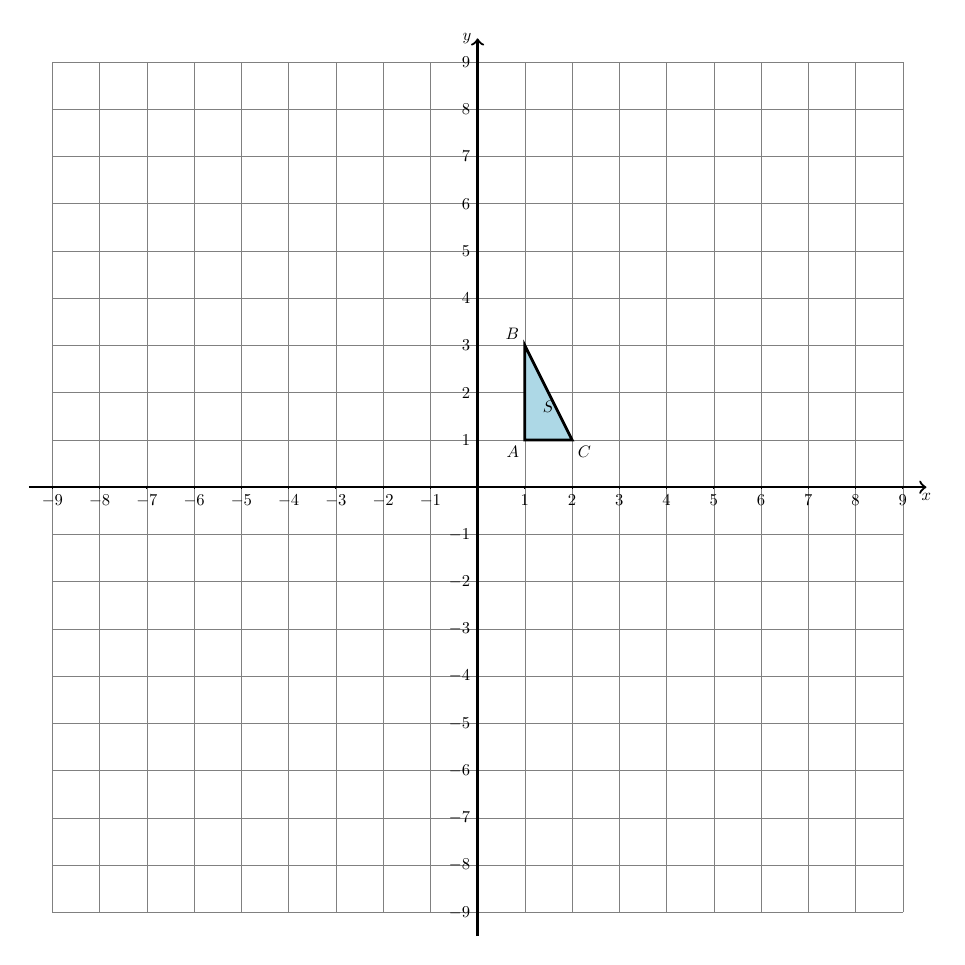
\begin{tikzpicture}[scale=0.6, transform shape]
    \definecolor{borderColour}{HTML}{000000}
    \definecolor{fillColourS}{HTML}{ADD8E6}

    \def\axisLimit{9}

    % Draw grid
    \draw[step=1cm,gray,very thin] (-\axisLimit,-\axisLimit) grid (\axisLimit,\axisLimit);

    % Draw axes
    \draw[thick,->] (-\axisLimit-0.5,0) -- (\axisLimit+0.5,0) node[anchor=north] {$x$};
    \draw[thick,->] (0,-\axisLimit-0.5) -- (0,\axisLimit+0.5) node[anchor=east] {$y$};

    % Label x-axis and y-axis
    \foreach \x in {-\axisLimit,...,-1,1,2,...,\axisLimit}
        \draw (\x cm,1pt) -- (\x cm,-1pt) node[anchor=north] {$\x$};
    \foreach \y in {-\axisLimit,...,-1,1,2,...,\axisLimit}
        \draw (1pt,\y cm) -- (-1pt,\y cm) node[anchor=east] {$\y$};

    % Define vertices of S
    \coordinate (A) at (1,1);
    \coordinate (B) at (1,3);
    \coordinate (C) at (2,1);

    % Draw S
    \draw[fill=fillColourS, draw=borderColour, line width=1pt] (A) -- (B) -- (C) -- cycle;
    \node[below left] at (A) {$A$};
    \node[above left] at (B) {$B$};
    \node[below right] at (C) {$C$};
    \node at (1.5,1.7) {$S$};

\end{tikzpicture}
\end{center}

\begin{enumerate}
    \item[(a)] Triangle $S$ is enlarged by scale factor 3, centre the origin $(0,0)$, to give triangle $S'$.\\
    Find the coordinates of the vertices of $S'$.

    \vspace{4cm}
    \answerplain{2}

    \item[(b)] Triangle $S'$ is then translated by the vector $\begin{pmatrix} -2 \\ 5 \end{pmatrix}$ to give triangle $S''$.\\
    Find the coordinates of the vertices of $S''$.

    \vspace{4cm}
    \answerplain{1}

    \item[(c)] The engineers need to know the final position of the corner of the panel that started at point $C$, after both transformations have been applied.\\
    Write down the coordinates of this point on triangle $S''$.

    \vspace{2cm}
    \answercoord{1}
\end{enumerate}
\end{question}
